\documentclass{beamer}

\usepackage{changepage}
\usepackage{subcaption}
%\usepackage[demo]{graphicx}
%\usepackage{floatrow}
\usepackage{sidecap}

\setbeamertemplate{caption}{\insertcaption}

\title{Amélioration du passage à l'échelle de l'espace pris par la blockchain Bitcoin}
\date{}%juin 2021}
\author{Benjamin Loison}

\addtobeamertemplate{navigation symbols}{}
{
    \usebeamerfont{footline}
    \usebeamercolor[fg]{footline}
    \hspace{1em}
    \insertframenumber/\inserttotalframenumber
}

\setbeamercolor{footline}{fg=blue}
\setbeamerfont{footline}{series=\bfseries}

\begin{document}

\frame{\titlepage}

%\begin{frame}
%\frametitle{Table of Contents}
%\tableofcontents
%\end{frame}

\begin{frame}

\frametitle{Introduction aux blockchains}

\begin{figure}
\centering
\begin{subfigure}{.5\textwidth}
  \centering
  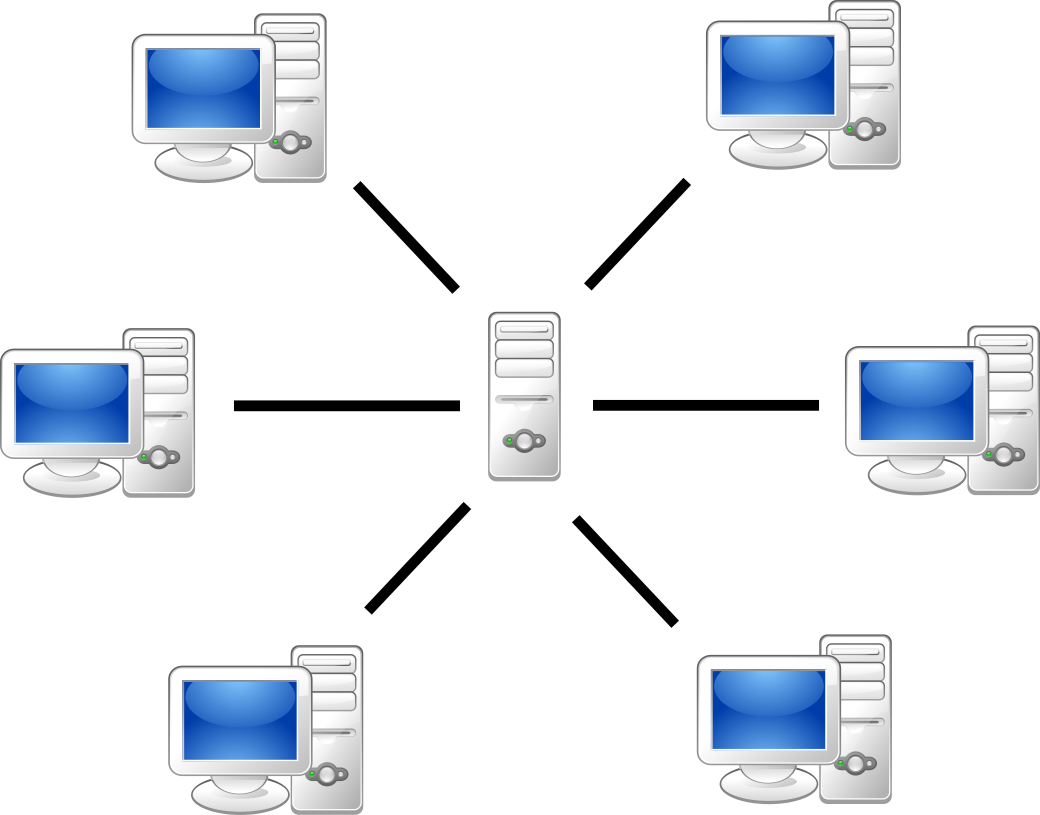
\includegraphics[width=.8\linewidth]{illustrationsSoutenance/clientServer.png}
  \caption{Réseau maître-esclave}
  \label{fig:sub1}
\end{subfigure}% if remove this comment it doesn't work anymore
\begin{subfigure}{.5\textwidth}
  \centering
  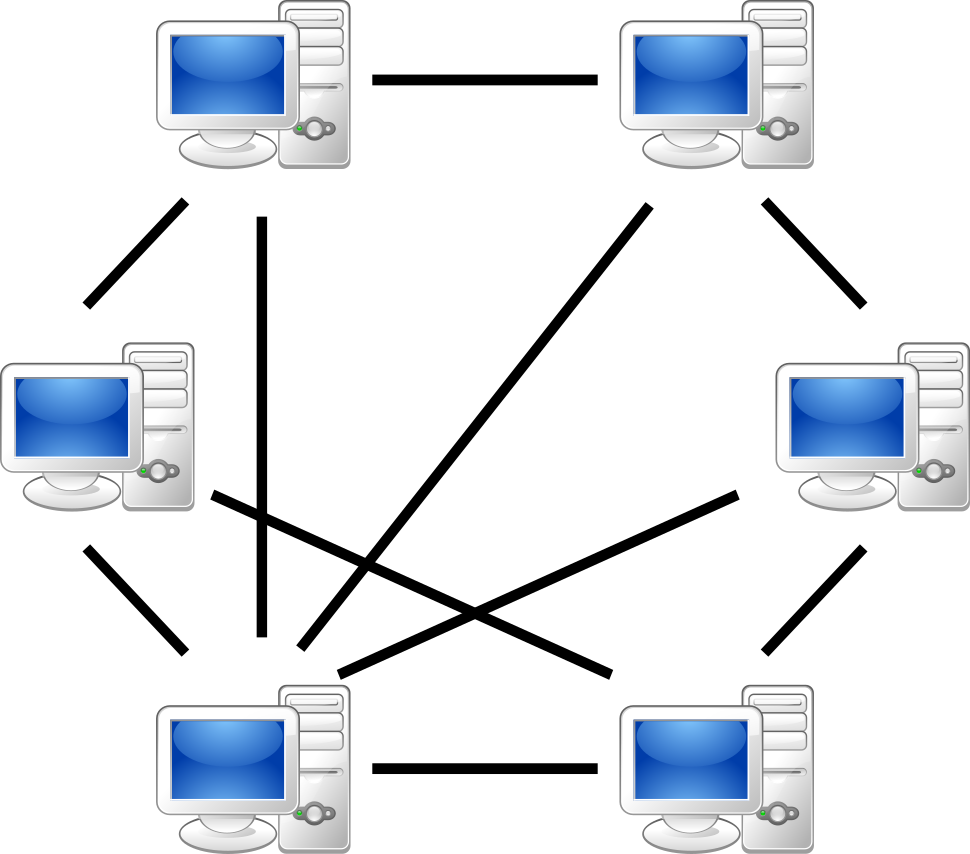
\includegraphics[width=.8\linewidth]{illustrationsSoutenance/P2P.png}
  \caption{Réseau pair-à-pair}
  \label{fig:sub2}
\end{subfigure}
\end{figure}
\end{frame}

%\newpage

\begin{frame}

\frametitle{Le problème du passage à l'échelle}

\begin{figure}[H]
		%\caption{Taille de la blockchain de Bitcoin en fonction du temps}
		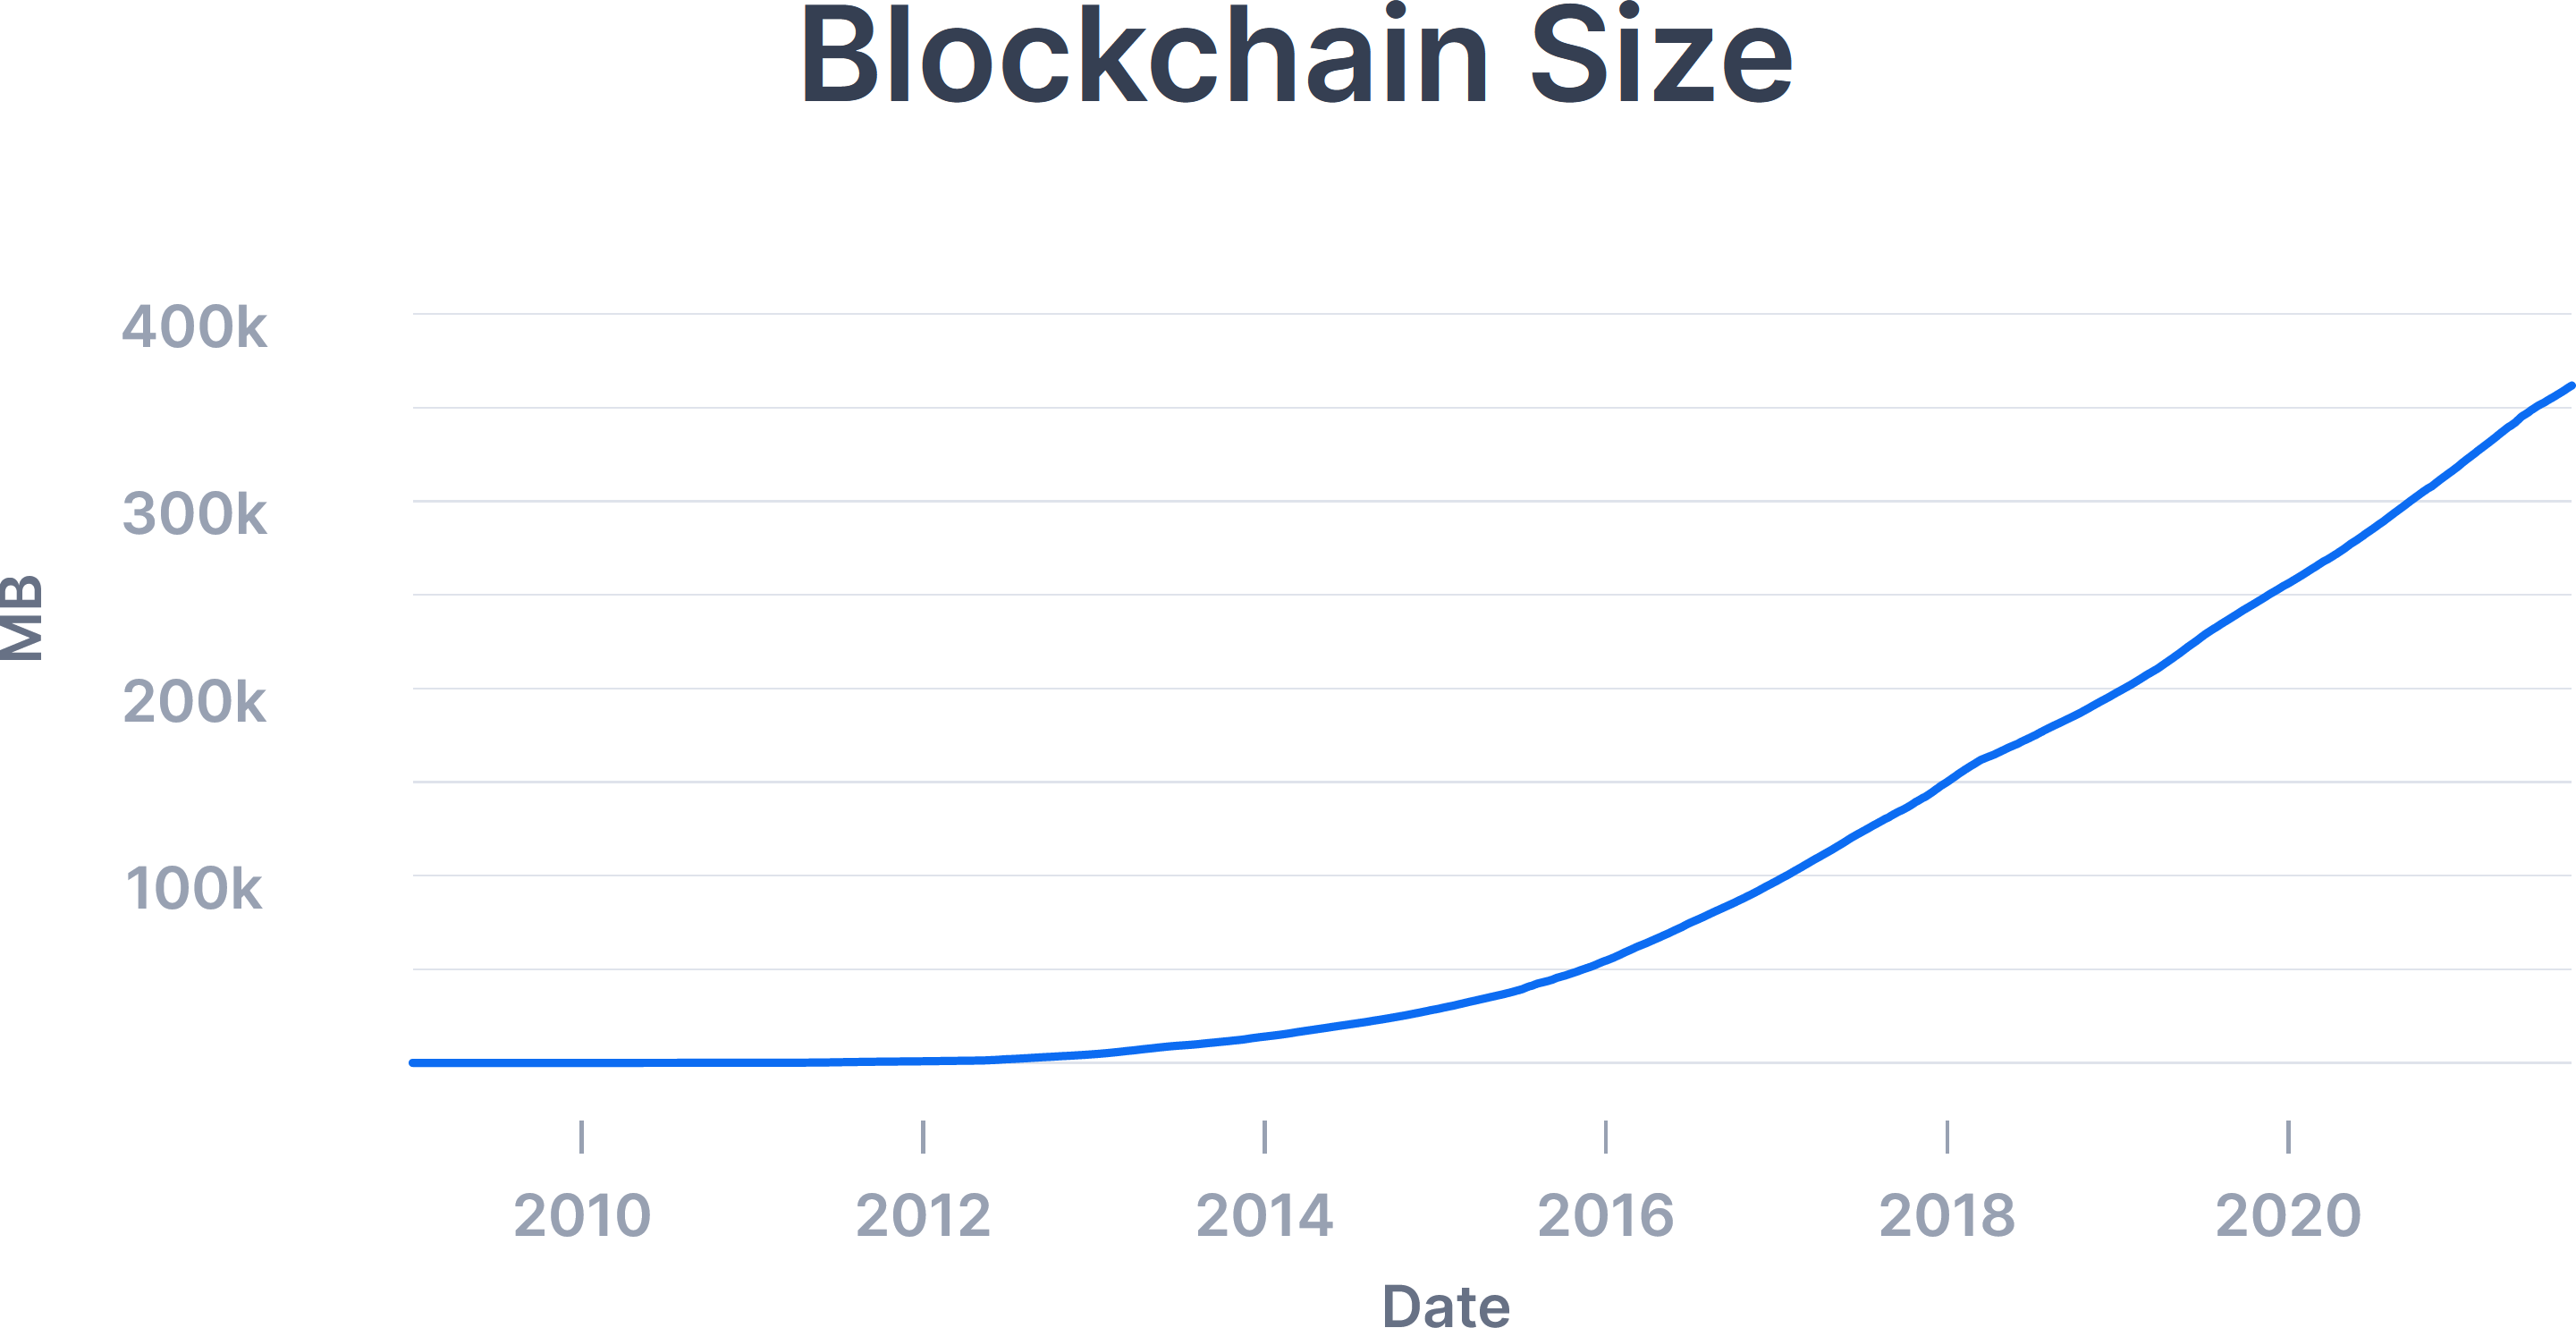
\includegraphics[width=\linewidth]{illustrationsSoutenance/blockchainSizeSourceless.png}
	\end{figure}

\end{frame}

\begin{frame}

\frametitle{L'idée du stage}

\begin{itemize}
	\item Mining in Logarithmic Space 2021 Aggelos Kiayias, Nikos Leonardos and Dionysis Zindros
\end{itemize}

\begin{figure}[H]
		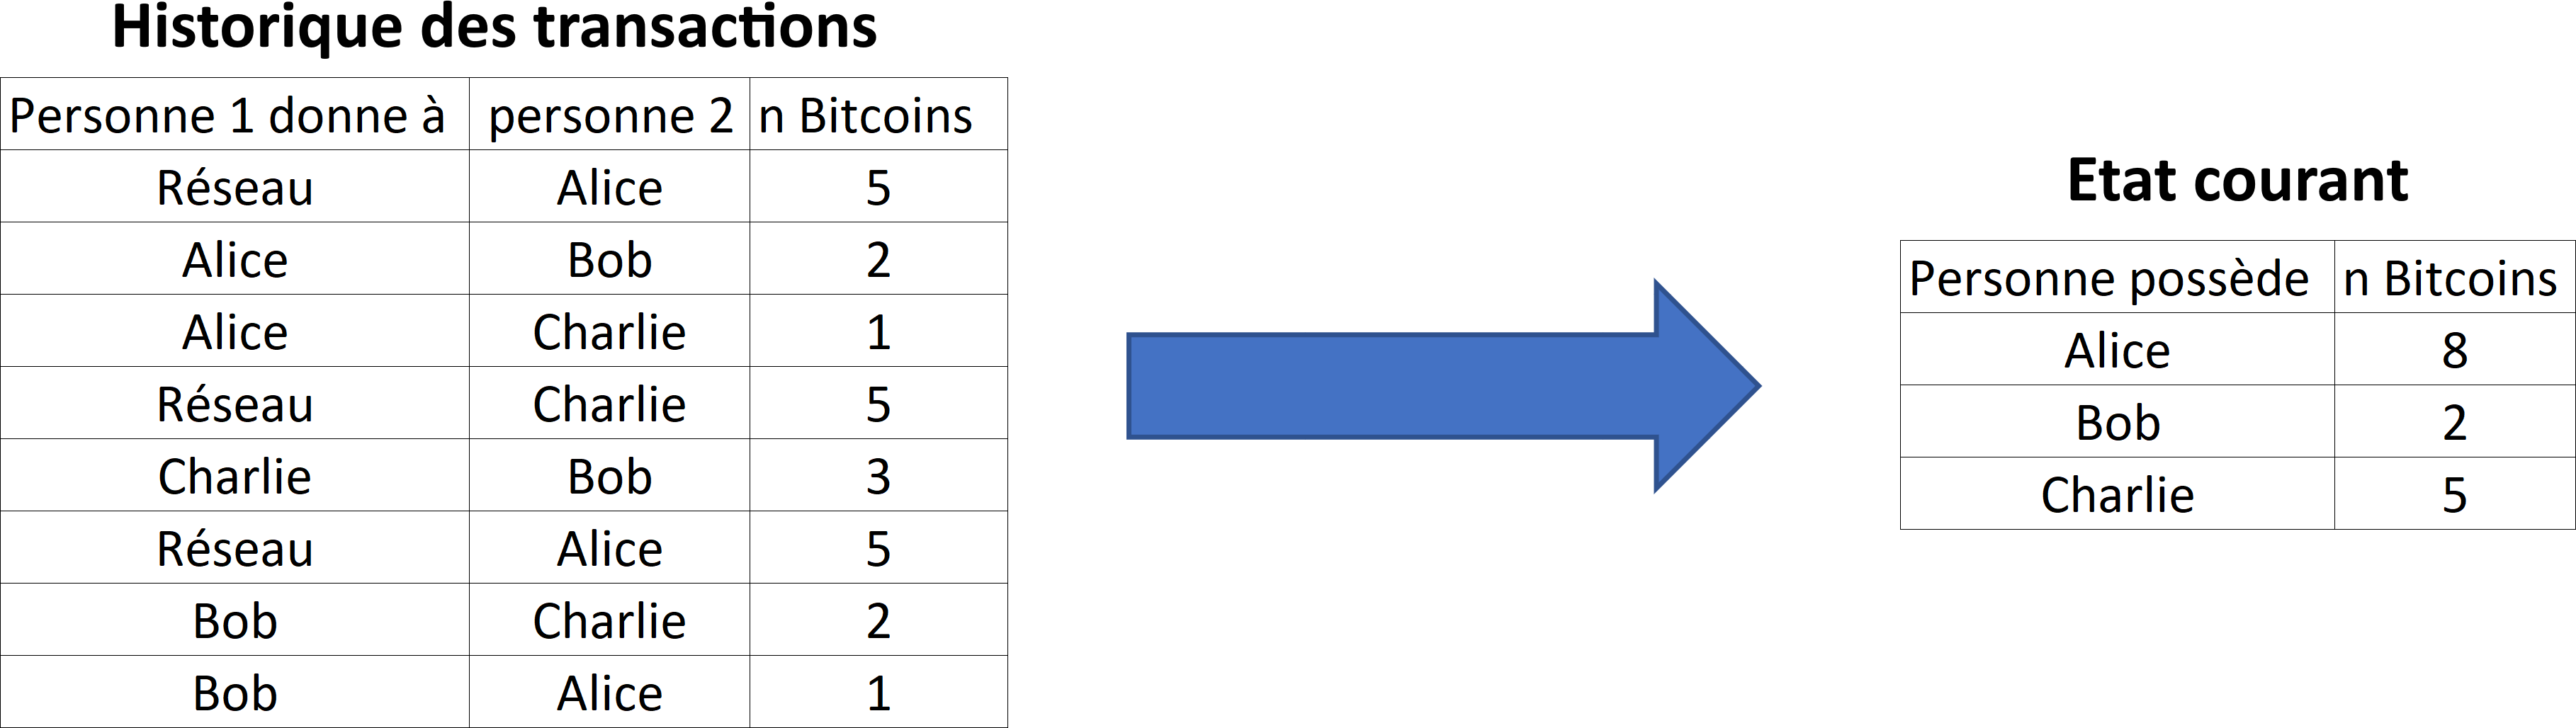
\includegraphics[width=\linewidth]{illustrationsSoutenance/ideaTitle.png}
	\end{figure}

\end{frame}


\begin{frame}

\frametitle{Le fonctionnement de Bitcoin}

\begin{figure}[H]
		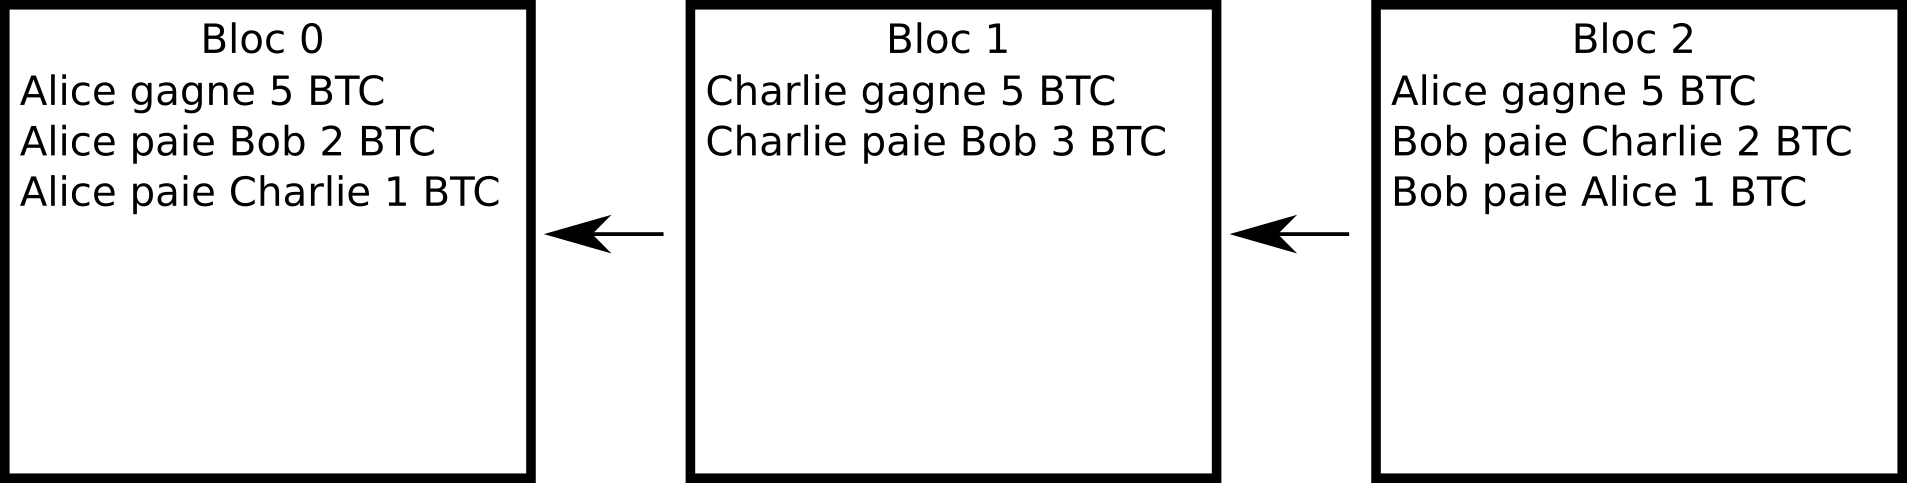
\includegraphics[width=\linewidth]{illustrationsSoutenance/blockchain.png}
	\end{figure}

\end{frame}


\begin{frame}

\frametitle{Miner des blocs}

Données:\\
\vspace{0.5cm}

Bloc 0 n\\
Alice gagne 5 BTC\\
Alice paie Bob 2 BTC\\
Alice paie Charlie 1 BTC\\

\vspace{0.5cm}
\begin{tabular}{| c | c |}
	\hline
   n     & haché SHA-256²\\ \hline
   0     & 6c7c2450bd52e950a3db47d8dc91cbdb04a792561759\dots \\ \hline
   1     & 6442a403b0cd2bac7b3af363a342769d1955f9851d65\dots \\ \hline
   \dots & \dots \\ \hline
   86    & 00e9d707e8f386a73d2455cfa9c06d618285f03e434a\dots\\
	\hline
 \end{tabular}

\end{frame}


\begin{frame}

\frametitle{Le problème du fork}

\begin{figure}[H]
		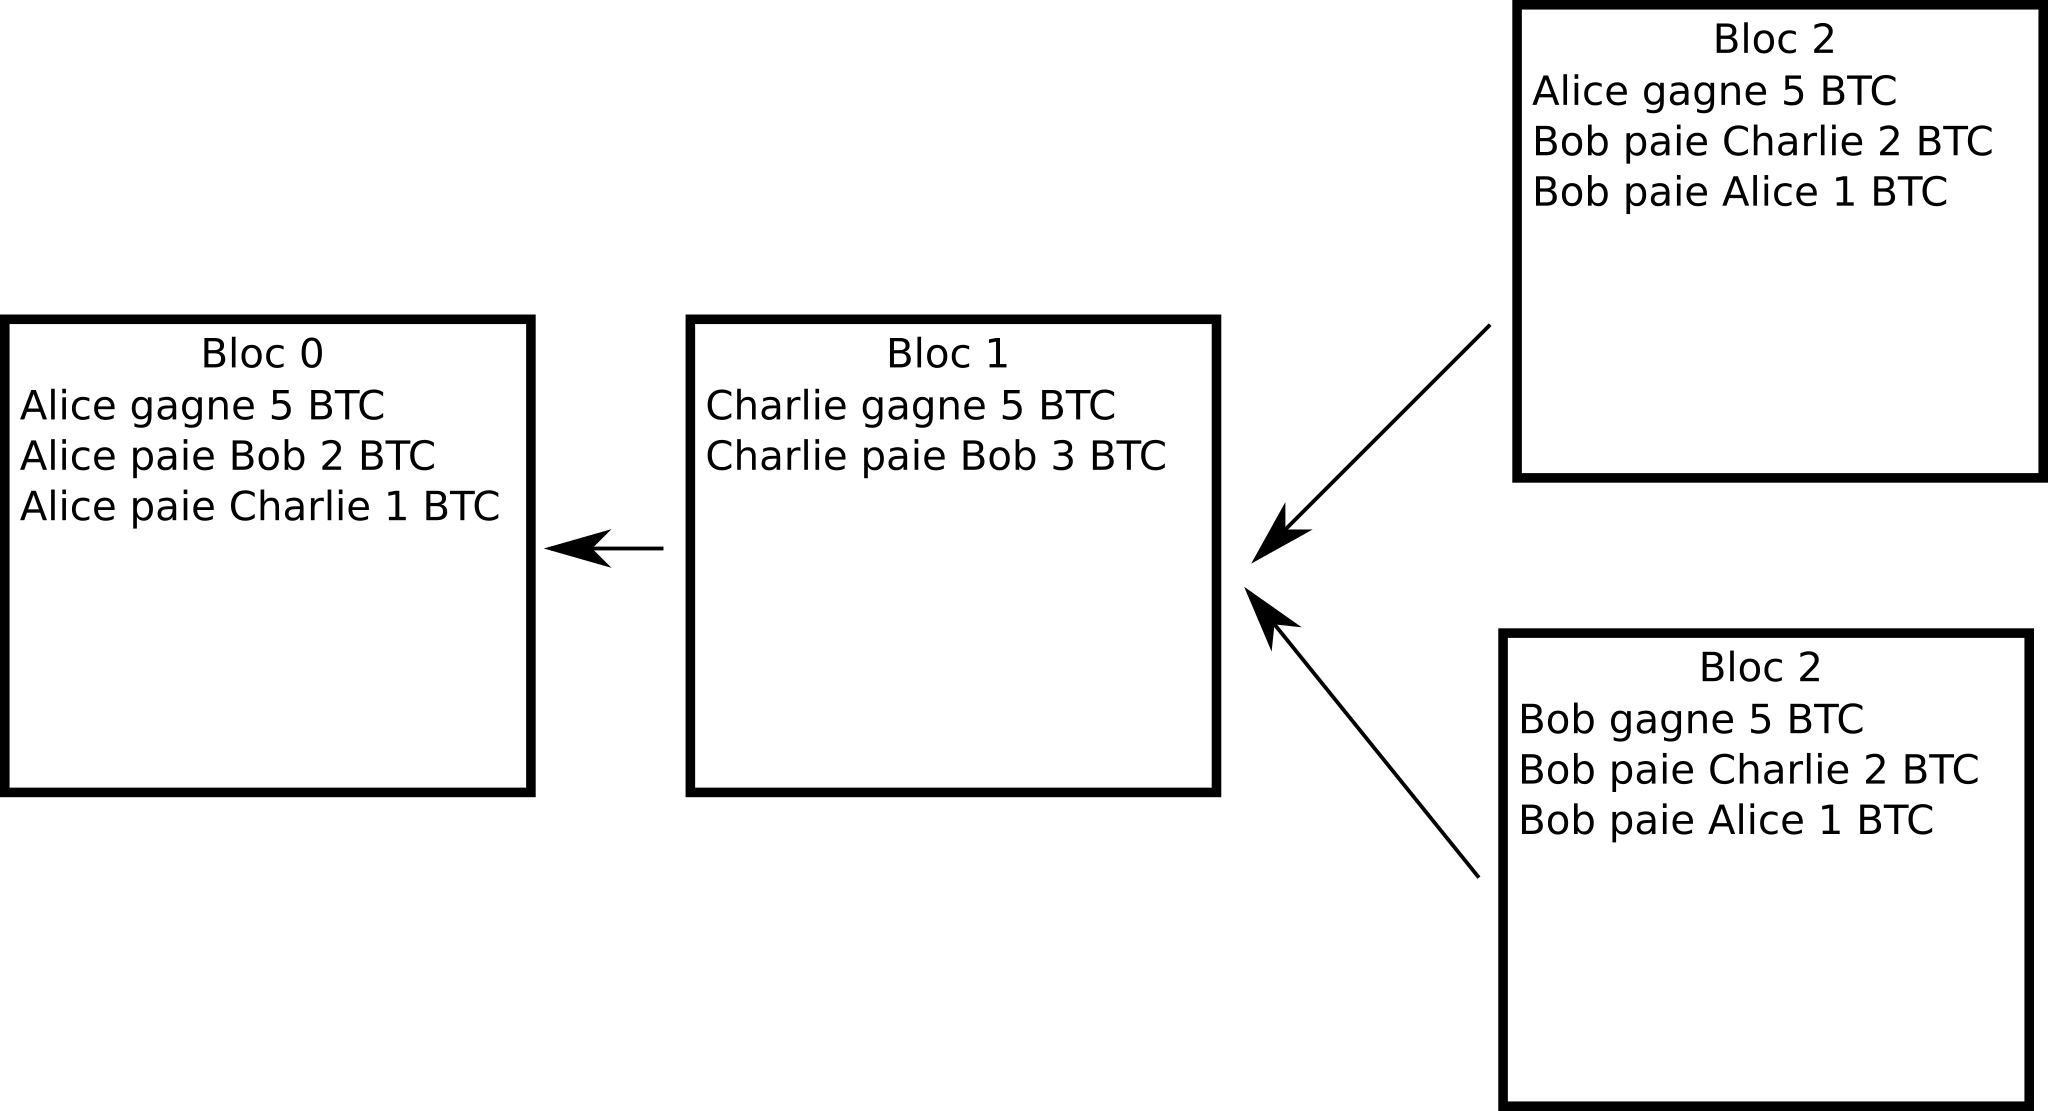
\includegraphics[width=\linewidth]{illustrationsSoutenance/fork.png}
	\end{figure}

\end{frame}


\begin{frame}

\frametitle{Le problème du fork}

\begin{figure}[H]
		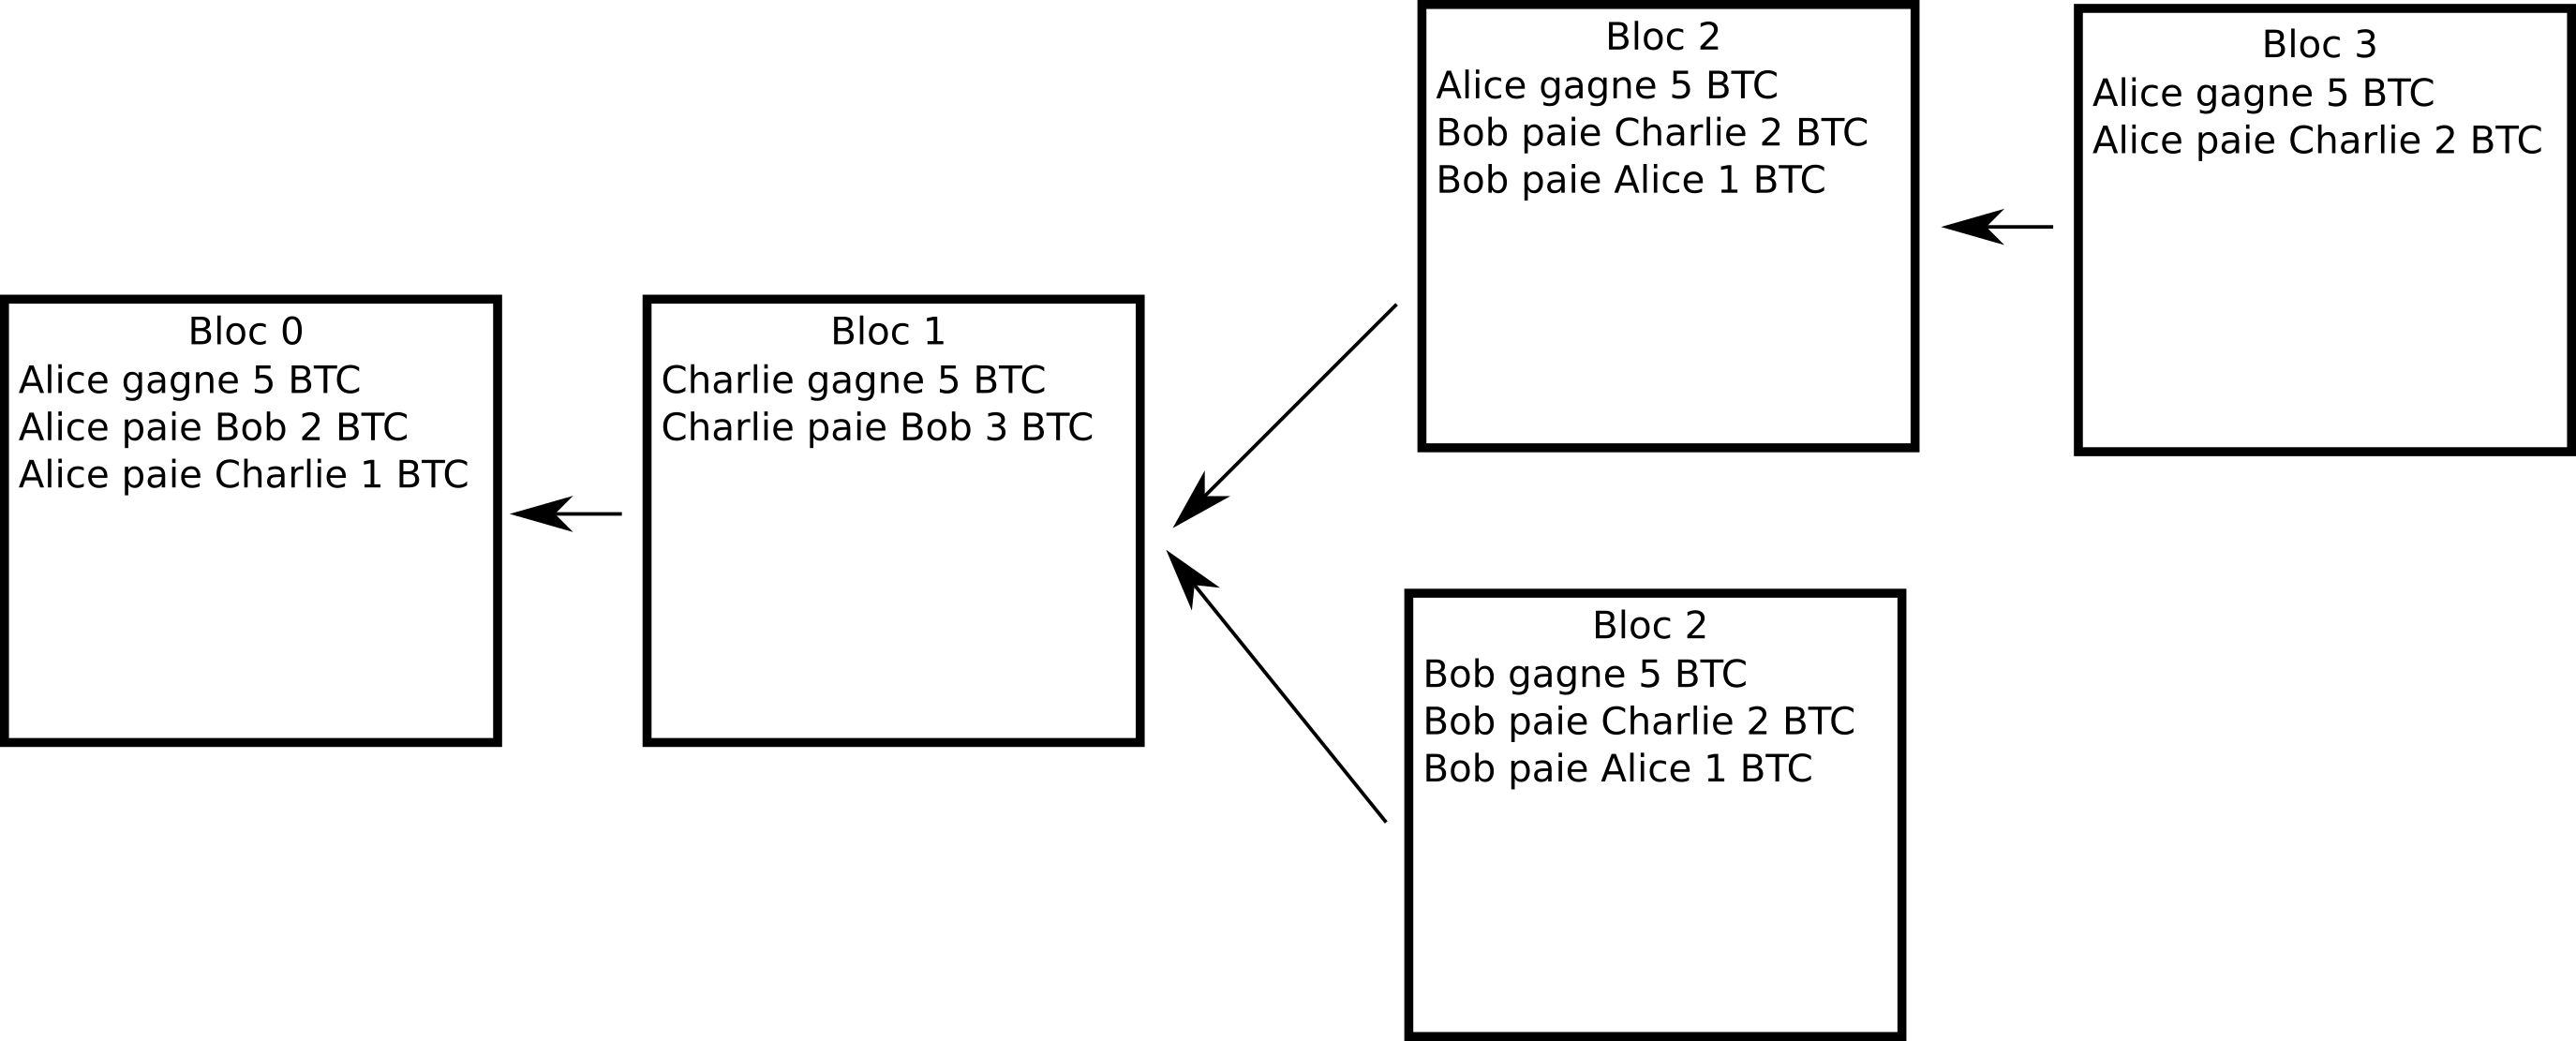
\includegraphics[width=\linewidth]{illustrationsSoutenance/forkContinue.png}
	\end{figure}

\end{frame}


\begin{frame}

\frametitle{Les atouts de la théorie}

\begin{figure}[H]
		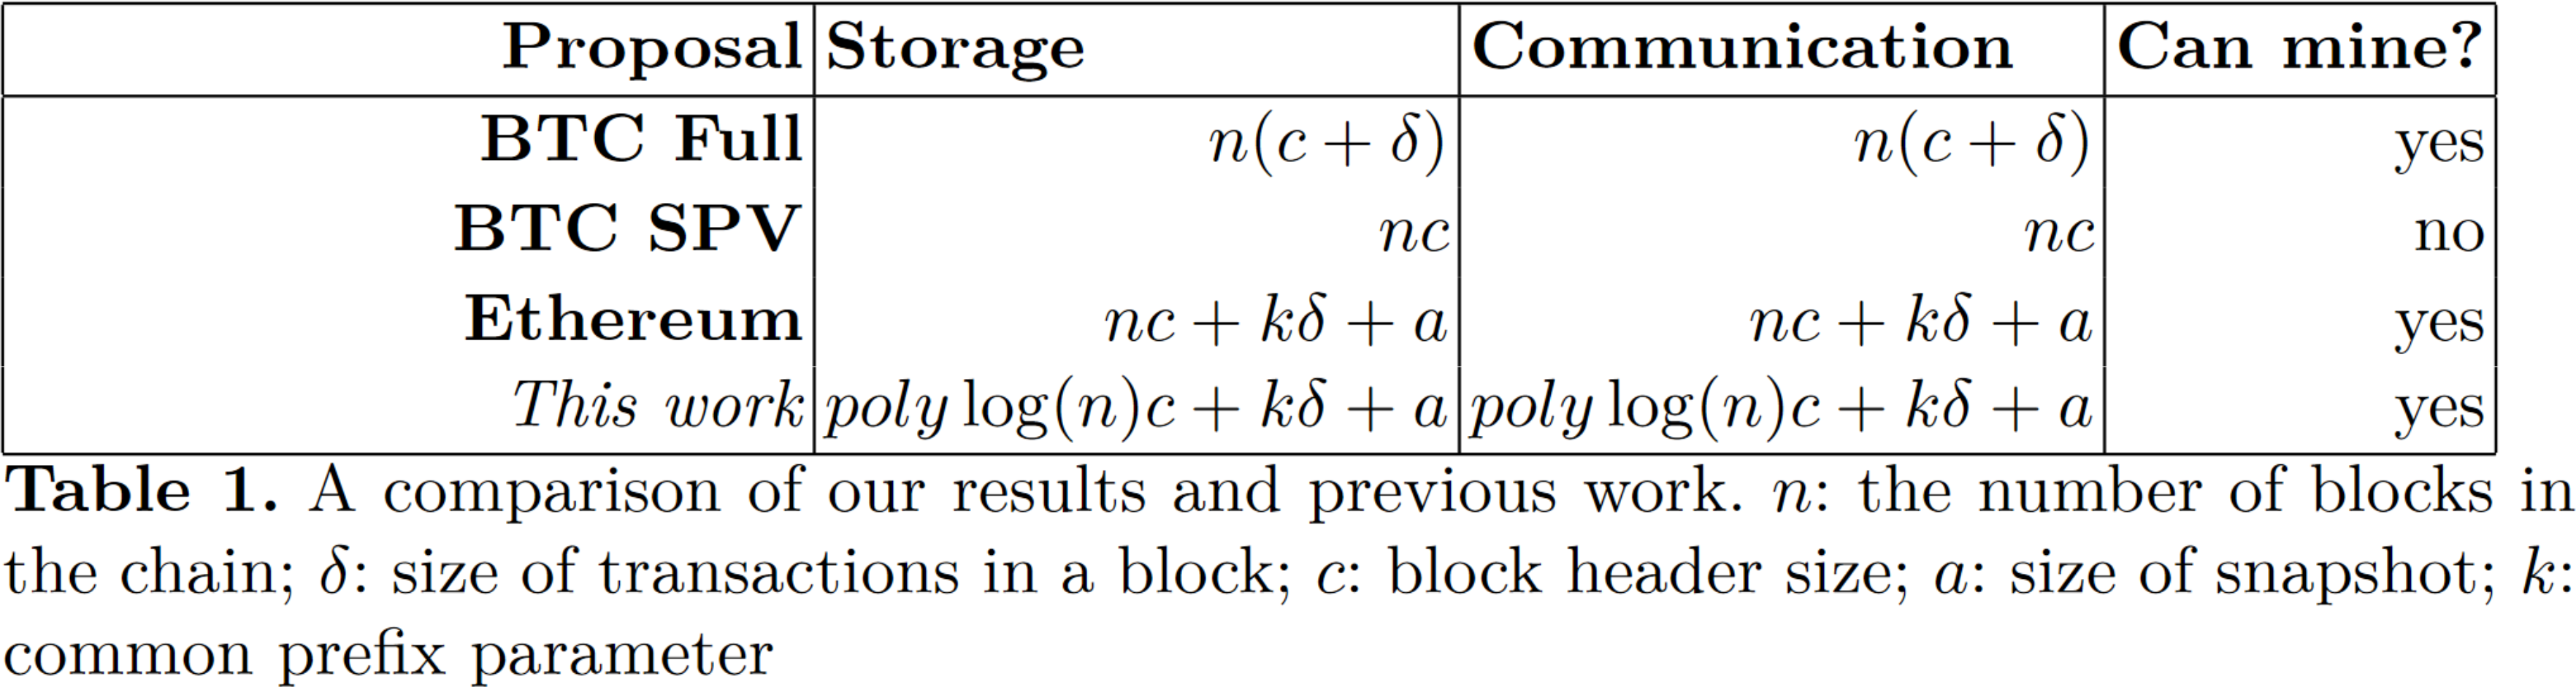
\includegraphics[width=\linewidth]{illustrations/tableauPage9.png}
		\caption{Extrait du tableau page 9 de "Mining in Logarithmic Space" (BTC signifiant Bitcoin)\\$n = 695 590$, $\delta$ entre 0 et 2 Mo, $c = 97$, $a = 4.24$ Go, $k = 6$}
	\end{figure}

\end{frame}

\begin{frame}

\frametitle{Le problème de l'interlink set}

\begin{figure}[H]
		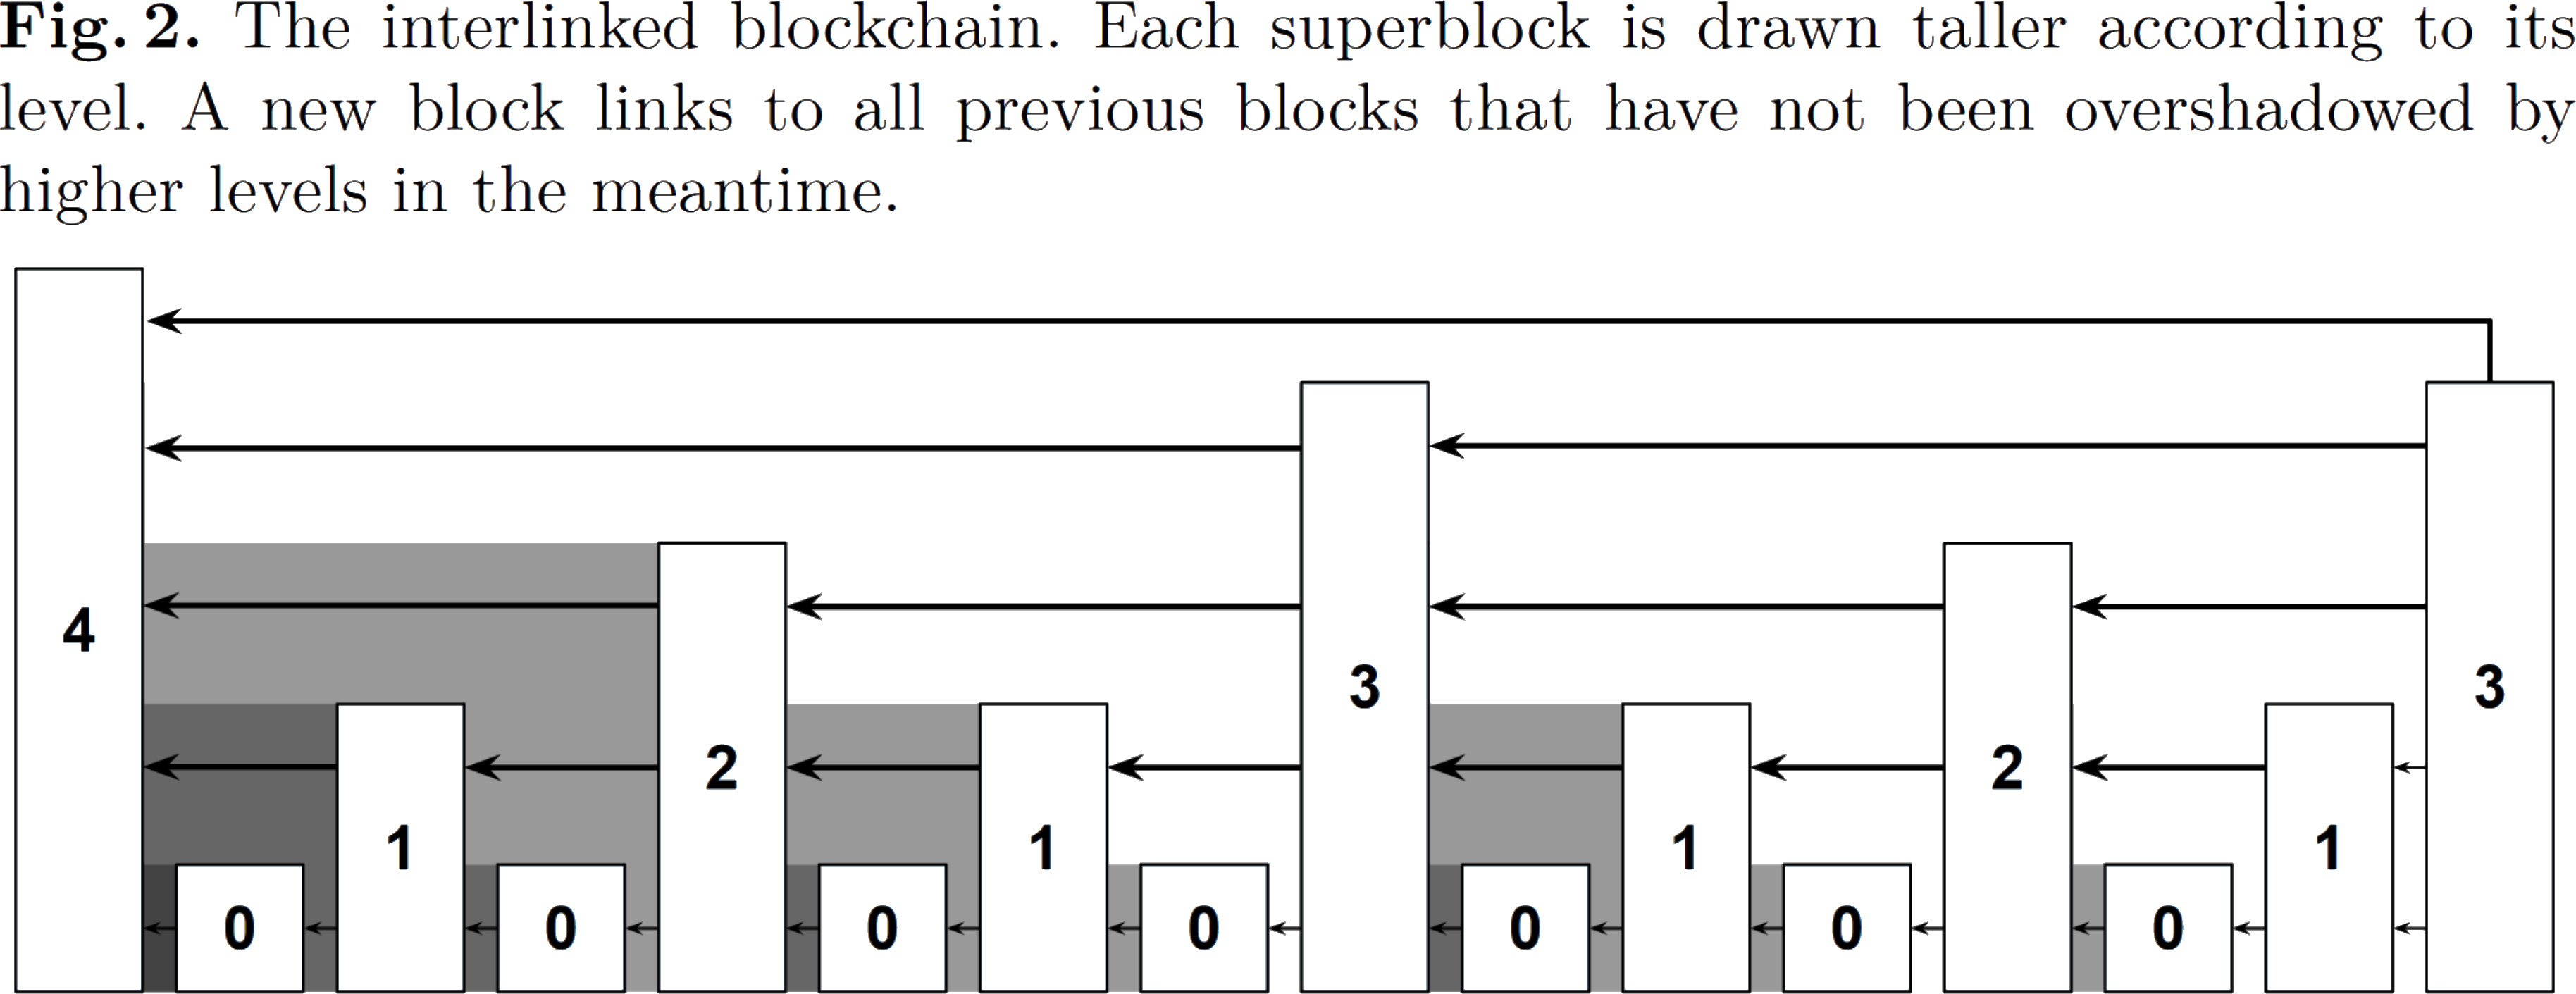
\includegraphics[width=\linewidth]{illustrations/interlinkSet.png}
		\caption{Ensemble de pointeurs de "Mining in Logarithmic Space" nécessaire à la bonne exécution de leur approche}
	\end{figure}

\end{frame}

\begin{frame}

\frametitle{Quelques statistiques}

\begin{figure}[H]
		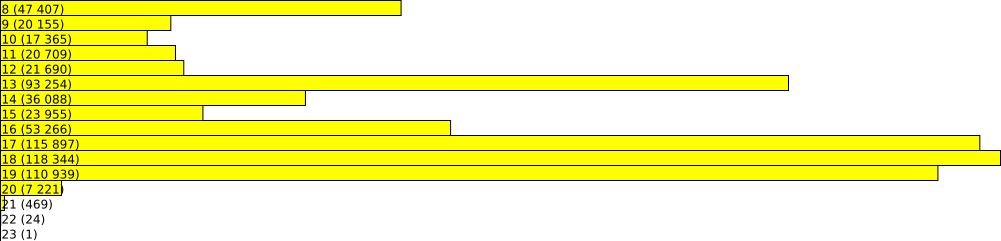
\includegraphics[width=\linewidth]{illustrations/hexaHashesStats.png}
		\caption{Répartition des hachés des blocs de Bitcoin par difficulté $m$ ($n$) où $m$ est le nombre de zéros hexadécimaux au début du haché et $n$ le nombre de hachés débutant précisément par $m$ zéros hexadécimaux}
	\end{figure}

\end{frame}

\begin{frame}

\frametitle{Quelques statistiques}

%\vspace{-0.25cm}
		%\hspace{-3cm}
%\begin{figure}[H]
		%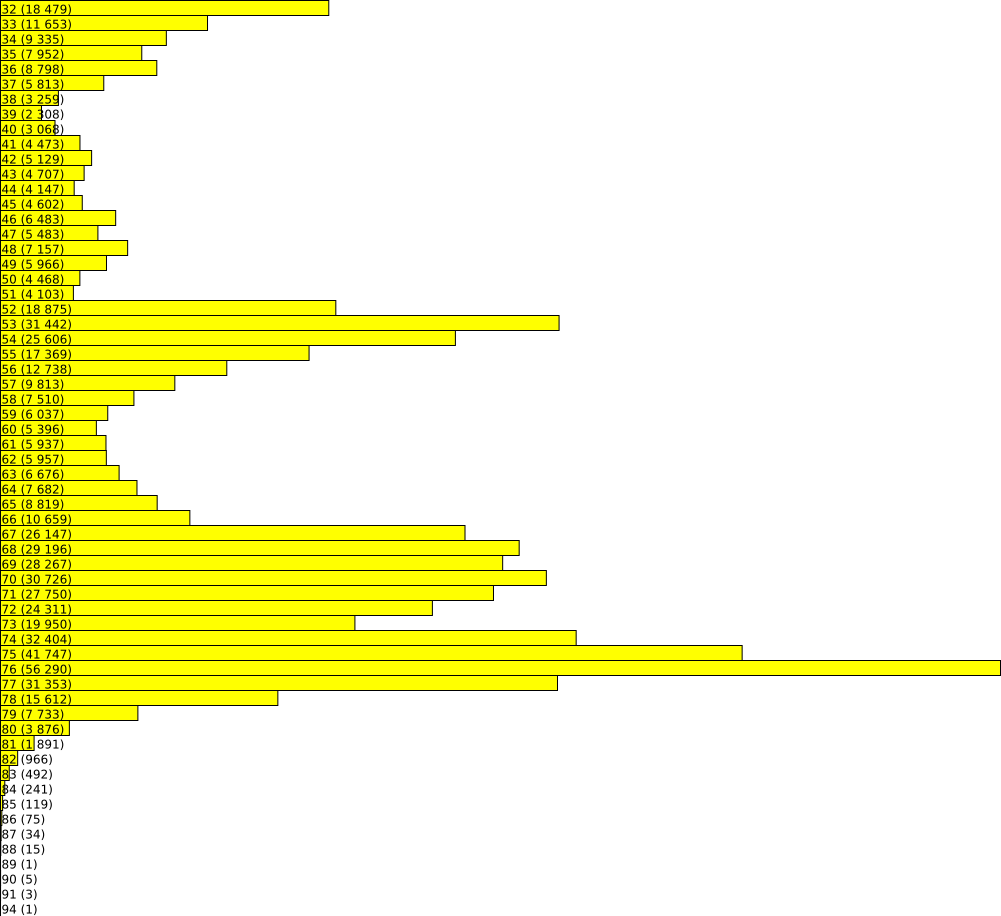
\includegraphics[width=0.85\linewidth]{illustrations/binHashesStats.png}
		%\hspace{5cm}
		%\vspace{-8cm}
		%\caption{Répartition des hachés des blocs de Bitcoin par difficulté $m$ ($n$) où $m$ est le nombre de zéros binaires au début du haché et $n$ le nombre de hachés débutant précisément par $m$ zéros binaires}
		%\begin{sidecaption}[fortoc]{title}[label]
%the body of the float
%\end{sidecaption}
	%\end{figure}
	
%	\begin{figure}
%\floatbox[{\capbeside\thisfloatsetup{capbesideposition={right,top},capbesidewidth=4cm}}]{figure}[\FBwidth]
%{\caption{A test figure with its caption side by side}\label{fig:test}}
%{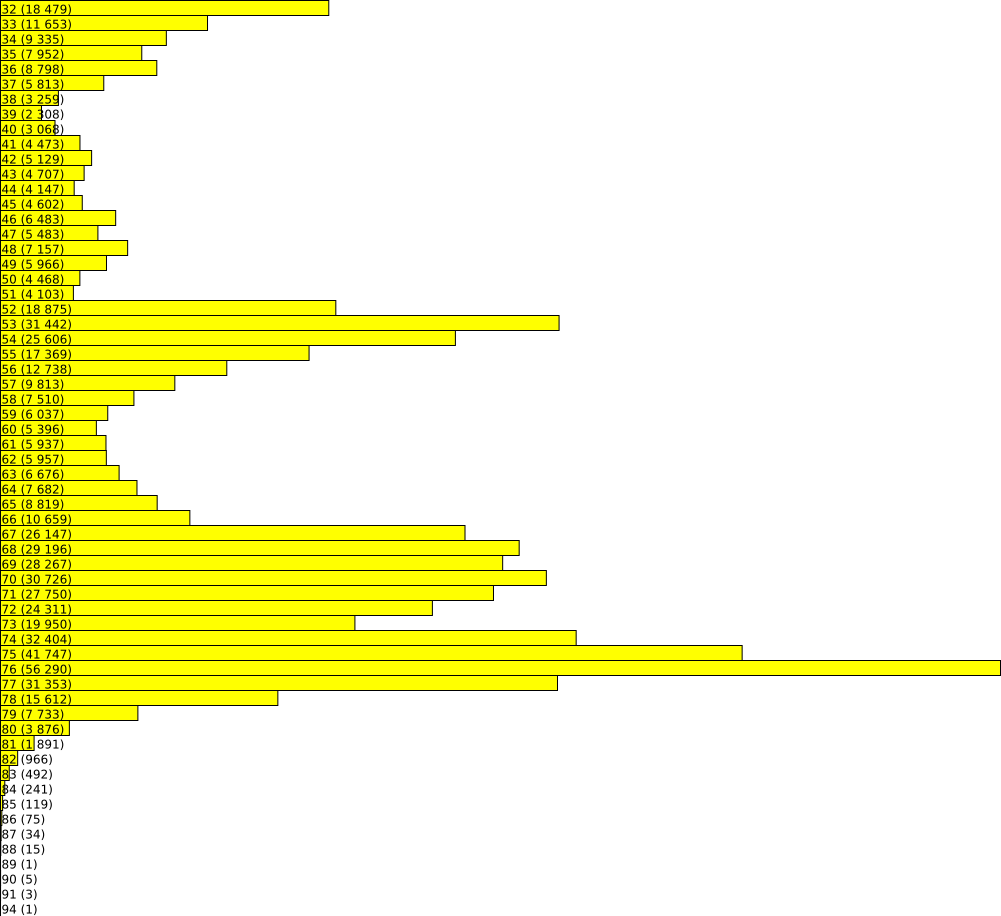
\includegraphics[width=5cm]{illustrations/binHashesStats.png}}
%\end{figure}

%\begin{SCfigure}
%    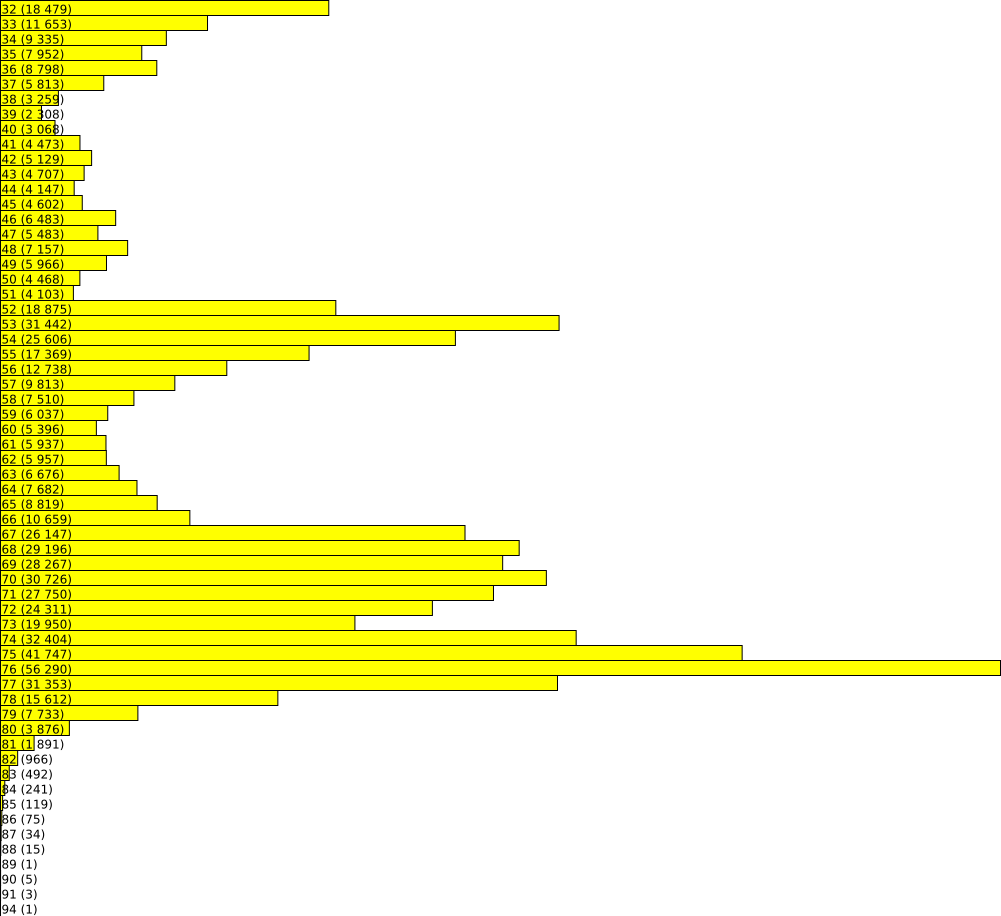
\includegraphics[width=5cm]{illustrations/binHashesStats.png}
%  \caption{Foo bar}
%\end{SCfigure}

\begin{figure}
      \begin{columns}
        \column{.8\linewidth}
        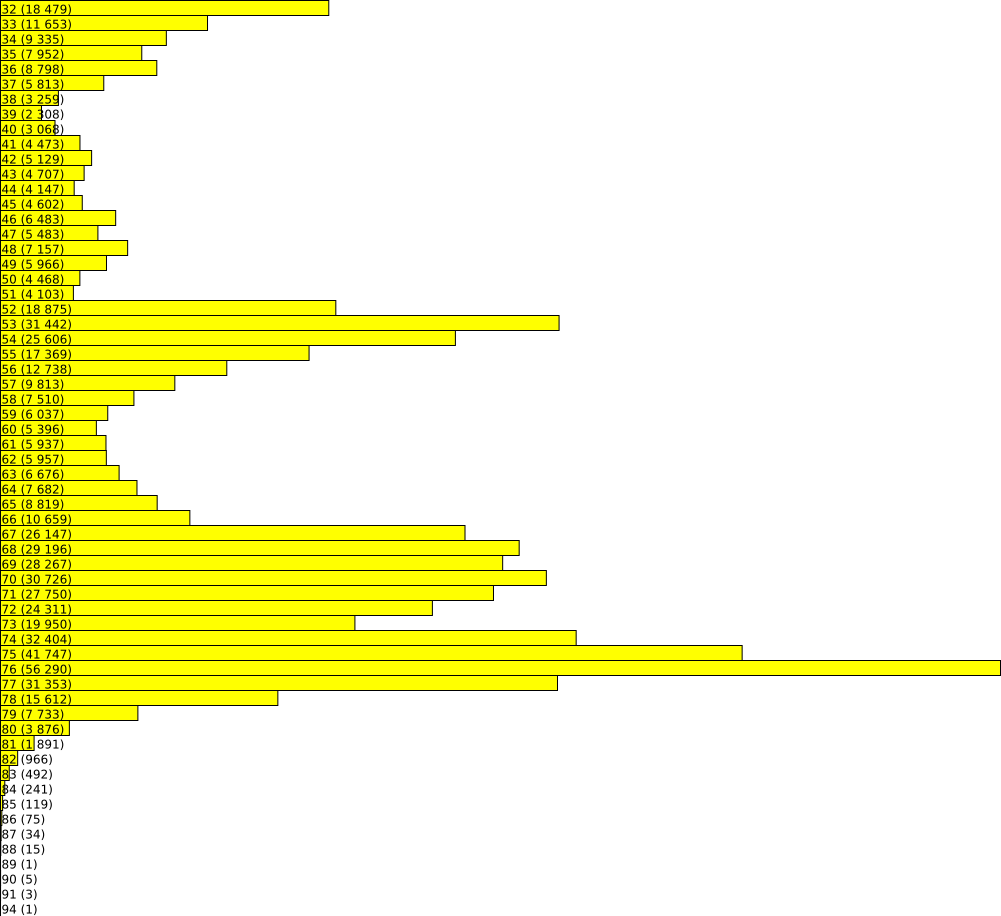
\includegraphics[width=\textwidth]{illustrations/binHashesStats.png}
        \column{.3\linewidth}
        \caption{Répartition des hachés des blocs de Bitcoin par difficulté $m$ ($n$) où $m$ est le nombre de zéros binaires au début du haché et $n$ le nombre de hachés débutant précisément par $m$ zéros binaires}
        \label{fig:example right}
      \end{columns}
    \end{figure}

%Test

\end{frame}

\begin{frame}

\frametitle{L'algorithme de compression}

%\vspace{-0.3cm}
\begin{figure}[H]
		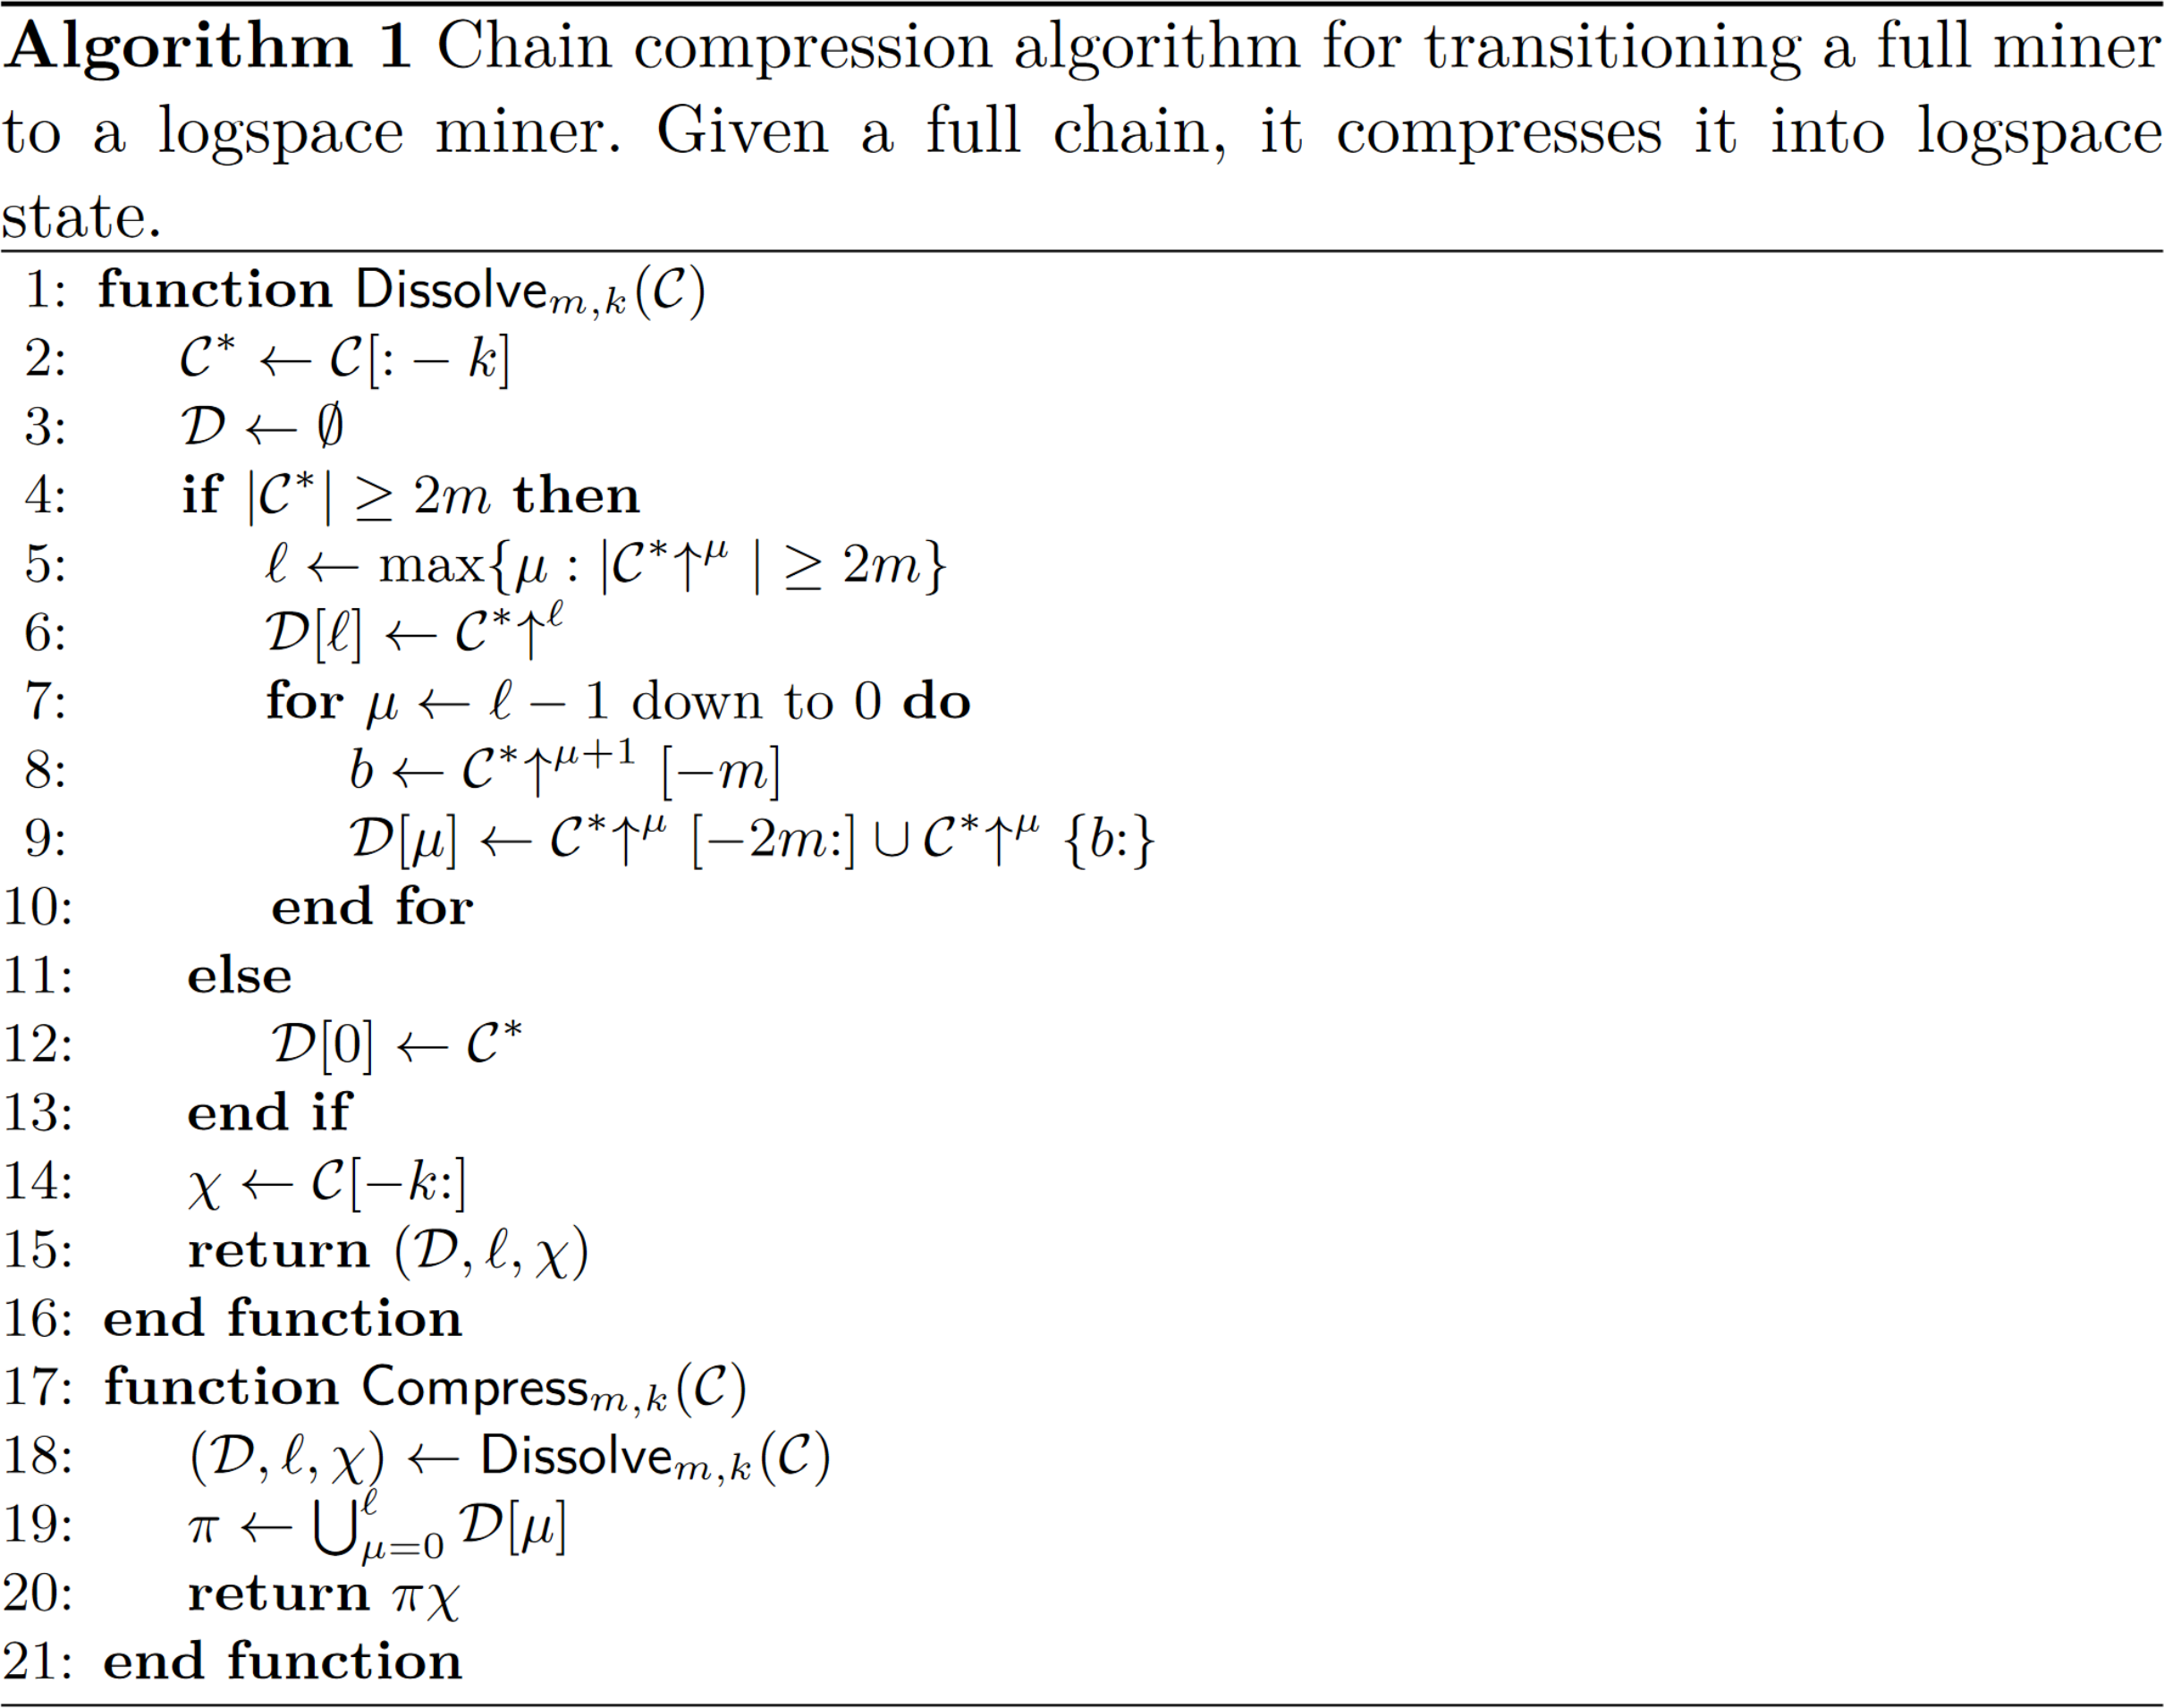
\includegraphics[width=0.7\linewidth]{illustrations/algo1.png}
		\caption{Algorithme 1 de "Mining in Logarithmic Space" permettant de compresser une blockchain.\\$C$ est la chaîne de blocs\\$C^*\uparrow^\mu$ désigne les blocs de niveau de difficulté exactement $\mu$ de $C^*$\\$C^*\uparrow^\mu\{b:\}$ désigne les blocs de $C^*\uparrow^\mu$ plus récents que le bloc $b$}
	\end{figure}

\end{frame}


\begin{frame}

\frametitle{Les résultats}

\begin{figure}[H]
		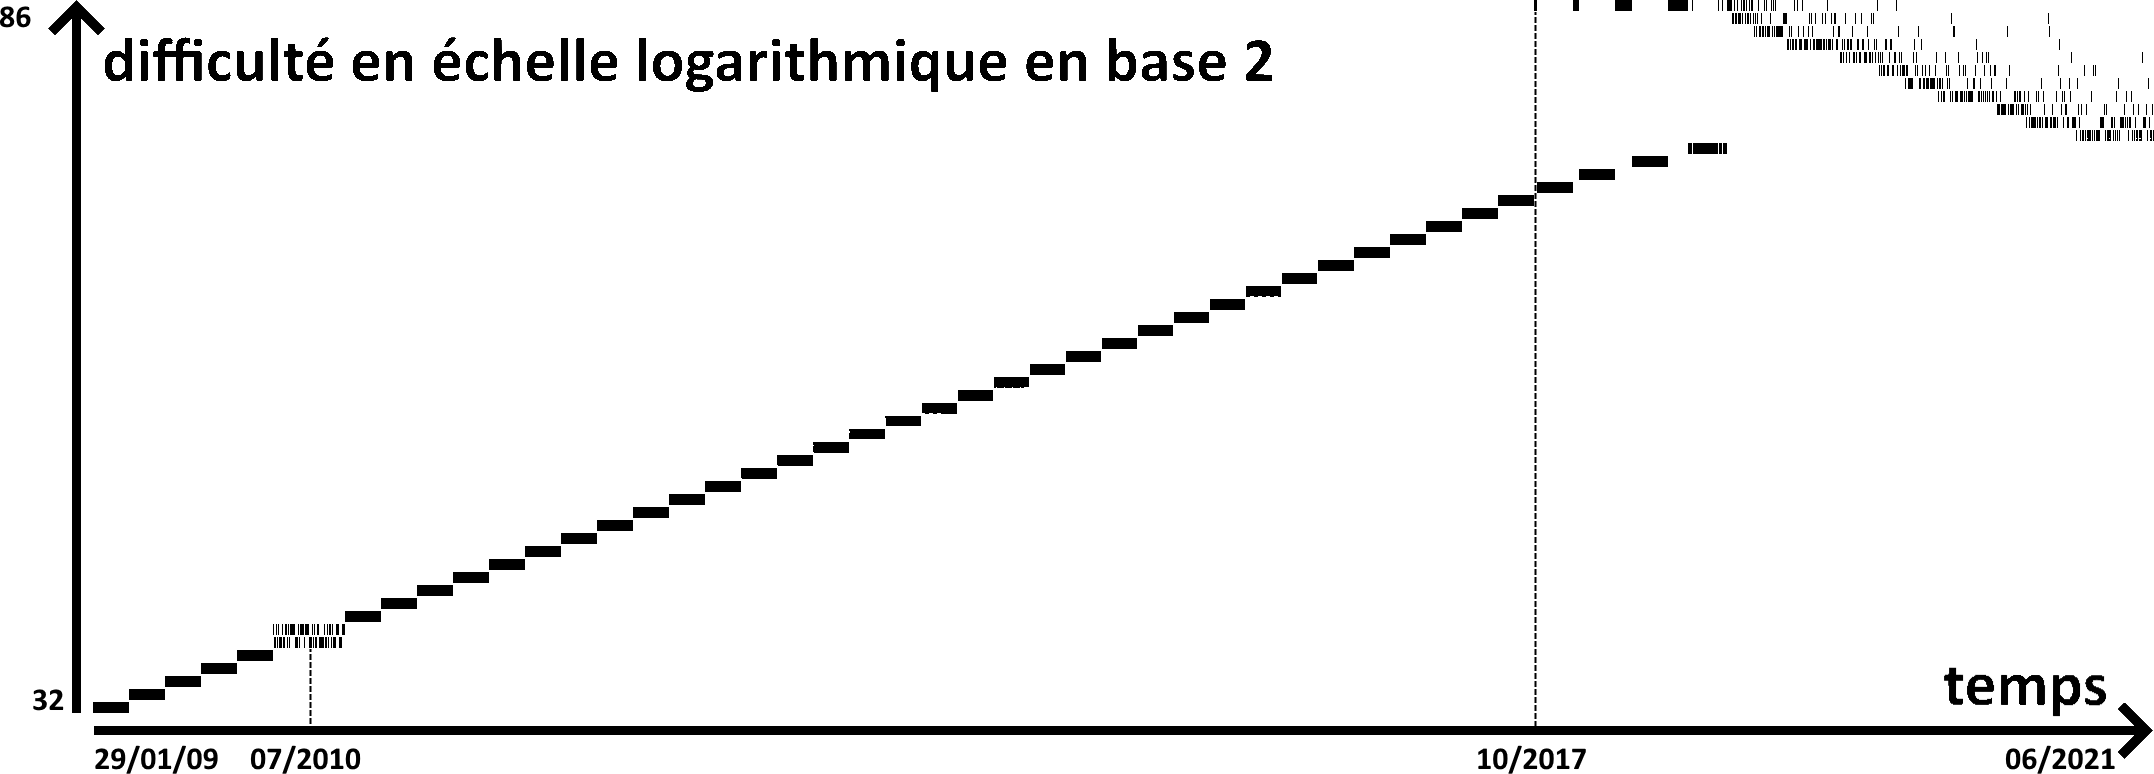
\includegraphics[width=\linewidth]{illustrations/piX.png}
		\caption{Répartition des hachés des blocs sélectionnés par l'algorithme 1, où chaque bloc a une largeur de 1 pixel}%$\pi\chi$, où chaque bloc a une largeur de 1 pixel}
	\end{figure}

\end{frame}


\begin{frame}

\frametitle{Sources des illustrations}

	\begin{itemize}
		\item Page 2: Wikipedia: peer-to-peer
		\item Page 3: Blockchain.com
	\end{itemize}
\end{frame}

\end{document}